% !TeX program = xelatex
% Overleaf: choose XeLaTeX and main.tex. All fonts are from TeX Live (Fandol).
\documentclass[UTF8,fontset=fandol,zihao=-4]{ctexart}
\usepackage[a4paper,left=20mm,right=20mm,top=20mm,bottom=20mm]{geometry}
\usepackage{graphicx,array,tabularx,tikz,enumitem,fancyhdr,xurl,hyperref,amsmath}
\usetikzlibrary{arrows.meta,positioning}
\hypersetup{hidelinks,pdftitle={实验1：Web服务器搭建与HTTP协议分析}}
\setlength{\parindent}{2em}
\setlength{\parskip}{5pt}
\setlength{\tabcolsep}{5pt}
\renewcommand{\arraystretch}{1.32}
\linespread{1.22}
\setlist[itemize]{leftmargin=1.5em,itemsep=3pt,topsep=3pt,parsep=0pt}
\setlist[enumerate]{leftmargin=1.8em,itemsep=4pt,topsep=3pt,parsep=0pt}
\pagestyle{fancy}
\fancyhf{}
\fancyhead[L]{\small 四川大学计算机学院、软件学院}
\fancyhead[R]{\small 计算机网络课程设计}
\fancyfoot[C]{\small\thepage}
\renewcommand{\headrulewidth}{0.3pt}
\setlength{\headheight}{16pt}

% Personal and course information confirmed by the user.
\newcommand{\studentname}{许盛凯}
\newcommand{\studentid}{2024141460445}
\newcommand{\majorname}{计算机科学与技术}
\newcommand{\classname}{计算机网络课程设计星期二34节}
\newcommand{\teachername}{陈黎}
\newcommand{\experimentdate}{2026 年 10 月 13 日}
\newcommand{\experimenttitle}{实验1：Web服务器搭建与HTTP协议分析}

\newlength{\bodywidth}
\setlength{\bodywidth}{\dimexpr\textwidth-19mm-4\tabcolsep-3\arrayrulewidth\relax}
\newsavebox{\reportcontentbox}
\newlength{\reportnaturalheight}
\newlength{\reportcontentlimit}
\setlength{\reportcontentlimit}{235mm} % 2 mm breathing room above the 237 mm frame.
\newcommand{\reportpage}[2]{%
  \clearpage
  \sbox{\reportcontentbox}{%
    \begin{minipage}[t]{\bodywidth}
    \vspace{2mm}\small\setlength{\parskip}{5pt}#2
    \end{minipage}}
  \setlength{\reportnaturalheight}{\dimexpr\ht\reportcontentbox+\dp\reportcontentbox\relax}
  \typeout{REPORTLAYOUT page=\thepage\space natural=\the\reportnaturalheight\space limit=\the\reportcontentlimit}
  \ifdim\reportnaturalheight>\reportcontentlimit
    \PackageError{report-layout}{Content exceeds the table frame on page \thepage}{Reduce image size or local spacing; do not hide overflowing content.}
  \fi
  \noindent\begin{tabular}{|m{19mm}|p{\bodywidth}|}
  \hline
  \raisebox{-112mm}[0pt][0pt]{\parbox{19mm}{\centering\small #1}} &
  \begin{minipage}[t][237mm][t]{\bodywidth}
  \noindent\usebox{\reportcontentbox}
  \end{minipage}\\\hline
  \end{tabular}
}
\newcommand{\subheading}[1]{\par\noindent\textbf{#1}\par\vspace{1mm}}
\newcommand{\qa}[2]{\par\noindent\textbf{#1}\par #2\par\vspace{2mm}}
\newcommand{\shot}[4][\linewidth]{%
  \par\noindent{\centering\includegraphics[width=#1]{assets/#2}\par}
  {\centering\footnotesize\textbf{图 #3}\quad #4\par}\vspace{2mm}
}
\newcommand{\code}[1]{\texttt{#1}}

\begin{document}

% Cover: matches the supplied reference's title, university wordmark,
% seal, large middle whitespace, underlined information and bottom date.
\hypersetup{pageanchor=false}
\begin{titlepage}
\thispagestyle{empty}
\begin{tikzpicture}[remember picture,overlay]
  \node[anchor=north,align=center,font=\songti\fontsize{12}{18}\selectfont]
    at ([yshift=-42mm]current page.north) {\experimenttitle};
  \node[anchor=north] at ([yshift=-59mm]current page.north)
    {
\includegraphics[width=98mm]{assets/scu.png}};
  \node[anchor=north] at ([yshift=-88mm]current page.north)
    {
\includegraphics[width=40mm]{assets/logo.png}};
  \node[anchor=north,font=\songti\fontsize{12}{18}\selectfont]
    at ([yshift=-201mm]current page.north) {%
    \renewcommand{\arraystretch}{1.0}%
    \begin{tabular}{@{}p{34mm}p{85mm}@{}}
    姓\quad 名： & \underline{\makebox[85mm]{\studentname}}\\[11mm]
    学\quad 号： & \underline{\makebox[85mm]{\studentid}}\\[11mm]
    专\quad 业： & \underline{\makebox[85mm]{\majorname}}\\[11mm]
    指导教师： & \underline{\makebox[85mm]{\teachername}}
    \end{tabular}};
  \node[anchor=north,font=\songti\fontsize{12}{18}\selectfont]
    at ([yshift=-278mm]current page.north) {\experimentdate};
\end{tikzpicture}
\null
\end{titlepage}
\setcounter{page}{1}
\hypersetup{pageanchor=true}

% Template front matter, retaining its original field names.
\begin{center}
  {\heiti\fontsize{16}{22}\selectfont 四川大学计算机学院、软件学院}\par
  \vspace{4mm}
  {\heiti\fontsize{24}{30}\selectfont 实\quad 验\quad 报\quad 告}
\end{center}
\vspace{2mm}
\noindent\small 学号：\studentid\quad 姓名：\studentname\quad 专业：\majorname\par
\noindent\small 班级：\classname\hfill 第\underline{\hspace{8mm}}周\par
\vspace{3mm}
\noindent\begin{tabularx}{\textwidth}{|m{23mm}|X|m{21mm}|m{36mm}|}
\hline
\centering 课程名称 & 计算机网络课程设计 & \centering 实验课时 & 第3—4节\\\hline
\centering 实验项目 & Web服务器搭建与HTTP协议分析 & \centering 实验时间 & \experimentdate\\\hline
\centering 实验目的 & \multicolumn{3}{p{\dimexpr\textwidth-23mm-4\tabcolsep-3\arrayrulewidth\relax}|}{%
  \begin{minipage}{\linewidth}\small\vspace{2mm}
  本实验为综合型实验，结合服务器配置与协议抓包，完成以下目标：
  \begin{enumerate}
    \item 在 Arch Linux 上配置 Apache HTTP Server，理解网站根目录、默认文档、监听地址和端口的作用。
    \item 通过浏览器访问自建静态页面，验证 URL 与本地文件的对应关系，确认页面由 HTTP 服务提供。
    \item 捕获指定测试页的 GET 请求和响应，依据实际首部分析版本、端点、状态码、类型与长度。
    \item 比较首次访问和普通刷新，解释 Conditional GET、缓存验证器及 304 响应的作用。
  \end{enumerate}\vspace{1mm}
  \end{minipage}}\\\hline
\centering 实验环境 & \multicolumn{3}{p{\dimexpr\textwidth-23mm-4\tabcolsep-3\arrayrulewidth\relax}|}{%
  \begin{minipage}{\linewidth}\small\vspace{2mm}
  \begin{tabularx}{\linewidth}{@{}lX@{}}
    操作系统 & Arch Linux（rolling），Linux 7.2.9-arch1-1，x86\_64\\
    硬件 & Intel Core i9-13900HX；TShark 检测内存 31,775 MiB\\
    本地服务器 & Apache HTTP Server 2.4.69（Unix），选择 Apache 方案\\
    浏览器 & Chromium 153.0.8010.52；独立实验配置，语言 zh-CN\\
    抓包与分析 & Wireshark/TShark 4.7.4；dumpcap 负责实际捕获\\
    抓包接口 & any；路由确认外网流量经 wlo1 发出\\
    本地站点 & \url{http://127.0.0.1:8086/}\\
    远程实验站点 & \code{gaia.cs.umass.edu}，TCP 80 端口
  \end{tabularx}
  \par 软件来源：从 Arch 官方仓库取得 Linux Apache、APR 和 APR-util 软件包，使用本机 Arch 公钥环验证包签名后在独立目录解包运行，不启用系统级 \code{httpd.service}。
  \par 环境、版本、包来源与校验记录随报告工程保存，见 \path{evidence/}；未提供的教学周保持空白。
  \vspace{2mm}\end{minipage}}\\\hline
\end{tabularx}

\reportpage{实验内容\\（算法、\\程序、\\步骤和\\方法）}{
\subheading{一、任务1：Apache 的获取、配置与验证}
\begin{enumerate}
  \item \textbf{选择与系统匹配的软件。}本机为 Arch Linux，选择 Apache 而非仅适用于 Windows 的 IIS。原文件夹的压缩包名称含 \code{win32}，不适用于本机，因此从 Arch 官方 extra 仓库获取 Linux 版 Apache 2.4.69 及 APR 依赖。
  \item \textbf{验证来源并隔离运行。}逐包核验软件包的独立签名，结果均为有效签名；只解包到本次实验的运行目录，使用 \code{LD\_LIBRARY\_PATH} 指向解包后的依赖库，不修改系统服务。
  \item \textbf{创建页面和配置。}制作 UTF-8 的 \code{index.html}，设置网页标题并写入姓名、学号、班级和实验内容。独立配置文件为 \path{experiment/httpd.conf}，日志保存于 \path{experiment/logs/}。
  \item \textbf{检查后启动。}使用 \code{httpd -f <配置路径> -t} 检查语法，实际输出 \code{Syntax OK}；随后以前台方式启动本次实例。\code{ss -ltn} 确认监听 \code{127.0.0.1:8086}，实际 GET 根路径得到 200。
\end{enumerate}
\shot{apache-config-crop.png}{1}{实际 Apache 版本、关键配置、语法检查与监听状态}
\subheading{关键配置的含义}
\begin{tabularx}{\linewidth}{|l|X|}\hline
\code{Listen 127.0.0.1:8086} & 只在本机 IPv4 回环地址的 TCP 8086 端口提供服务，避免直接暴露到局域网。\\\hline
\code{DocumentRoot} & 确定 URL 路径映射的起始目录，必须与 \code{Directory} 的访问授权范围一致。\\\hline
\code{DirectoryIndex index.html} & 访问目录根路径时查找并返回默认首页。\\\hline
\code{Require all granted} & 允许访问指定站点目录。本目录另用 \code{Options -Indexes} 关闭目录索引，并用 \code{AllowOverride None} 禁止 .htaccess 覆盖。\\\hline
\end{tabularx}
}

\reportpage{（接上）\\实验内容}{
\subheading{二、自建默认首页与访问结果}
\shot[0.82\linewidth]{apache-browser.png}{2}{真实 Chromium 窗口访问自建站点，地址栏与个人信息同时可见}
\subheading{站点参数记录}
\begin{tabularx}{\linewidth}{|l|X|}\hline
网站根目录 & \path{/home/assumeengage/NC_cl/}\newline 实验1\path{_Overleaf/experiment/www}\\\hline
默认首页文件 & \code{index.html}\\\hline
监听地址与端口 & \code{127.0.0.1:8086}（非默认 HTTP 端口）\\\hline
实际访问 URL & \url{http://127.0.0.1:8086/}\\\hline
访问方式与结果 & 浏览器发出 \code{GET / HTTP/1.1}，Apache 返回 200，正文显示完整实验信息。\\\hline
\end{tabularx}
\par URL 中 \code{127.0.0.1} 指向当前计算机，浏览器和服务器可以运行在同一台机器上。路径 \code{/} 先映射到网站根目录，再由 \code{DirectoryIndex} 选择该目录下的 \code{index.html}；不是直接双击 HTML 文件，也不是使用 \code{file://} 打开。
\par HTTP 未显式指定端口时通常访问 TCP 80；本实验改用 8086，因此 URL 中必须写出 \code{:8086}。响应头中的 Apache 标识、浏览器地址栏以及访问日志，共同证明访问的是本次配置的服务。
\subheading{访问过程示意}
\begin{center}
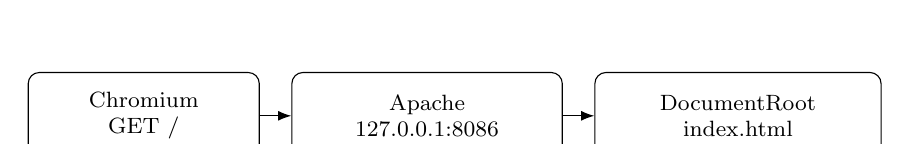
\begin{tikzpicture}[>=Latex,node distance=4mm, every node/.style={font=\footnotesize,align=center}]
\node[draw,rounded corners,text width=27mm,minimum height=11mm] (b) {Chromium\\GET /};
\node[draw,rounded corners,text width=32mm,minimum height=11mm,right=of b] (s) {Apache\\127.0.0.1:8086};
\node[draw,rounded corners,text width=34mm,minimum height=11mm,right=of s] (f) {DocumentRoot\\index.html};
\draw[->] (b)--(s);\draw[->] (s)--(f);
\end{tikzpicture}
\end{center}
}

\reportpage{（接上）\\实验内容}{
\subheading{三、任务2：基本 HTTP 抓包过程与证据}
\par 在隔离浏览器中清除实验资源缓存，明确使用 \code{http://} 访问指定地址。先开启 dumpcap 捕获，再打开页面；未使用 HTTPS 代替目标 HTTP 页面，未导入日常浏览器 Cookie 或登录状态。
\noindent\url{http://gaia.cs.umass.edu/wireshark-labs/HTTP-wireshark-file1.html}
\par 捕获过滤器为 \code{host 128.119.245.12 and tcp port 80}，Wireshark 显示过滤器为 \code{http}。完整捕获含 38 帧，其中 10 帧被识别为 HTTP；请求帧8和响应帧12构成目标页面的一组完整交换。
\shot{http-file1-request-crop.png}{3}{file1 的 GET 请求（帧8）；请求行、语言、编码及响应关联可见}
\shot{http-file1-response-crop.png}{4}{file1 的 200 OK 响应（帧12）；版本、长度、类型与修改时间可见}
\par\footnotesize 图3—8均为同一真实抓包的 Wireshark 截图；响应图仅保留报文详情区域，其余图裁去无关窗格和空白，未改写字段。完整原图与 pcapng 同时保留。
}

\reportpage{（接上）\\实验内容}{
\subheading{四、任务3：清除缓存后的首次访问}
\noindent\url{http://gaia.cs.umass.edu/wireshark-labs/HTTP-wireshark-file2.html}
\par 访问 file2 前通过浏览器的缓存清除接口清空浏览器缓存，随后正常导航到上述原始 URL。首次请求为帧20，响应为帧23；没有添加查询参数或手工注入缓存验证首部。
\shot{http-file2-first-request-crop.png}{5}{file2 首次 GET（帧20），没有 If-Modified-Since 或 If-None-Match}
\shot{http-file2-first-response-crop.png}{6}{首次响应（帧23），状态200、实体371字节，并给出 Last-Modified 与 ETag}
\par\footnotesize 首次请求与响应的 TCP 四元组为 \code{10.20.41.171:57438} 与 \code{128.119.245.12:80}，Wireshark 标记为 \code{tcp.stream == 1}。
}

\reportpage{（接上）\\实验内容}{
\subheading{五、任务3：紧接普通刷新后的缓存验证}
\par 首次页面加载完成后，立即对相同 URL 执行一次普通刷新，不执行强制刷新，也不再次清空缓存。浏览器自行加入验证器，帧28为第二次 GET，帧29为其响应；两次访问均使用 \code{tcp.stream == 1}。
\shot{http-file2-conditional-request-crop.png}{7}{第二次 GET（帧28），同时携带 If-None-Match、If-Modified-Since 和 max-age=0}
\shot{http-file2-304-response-crop.png}{8}{第二次响应（帧29），网络状态为304 Not Modified，没有实体正文}
\par\footnotesize 帧29没有 \code{Content-Length}、\code{Content-Type} 或 \code{File Data} 项。浏览器仍能显示首次取得的页面正文，这是使用本地缓存的结果，不能据此认为服务器再次发送了完整 HTML。
}

\reportpage{（接上）\\实验内容}{
\subheading{六、资料查阅与实际排障}
\qa{1. 抓包接口不可用：权限问题}{
\textbf{现象：}运行 \code{tshark -D} 时只显示远程捕获插件，并提示 \code{Couldn't run dumpcap in child process: Permission denied}，不能开始本机抓包。
\par\textbf{排查依据：}本机 \code{/usr/bin/dumpcap} 的所属组为 \code{wireshark}，权限为 \code{rwxr-xr--}，已具有 \code{cap\_net\_admin}、\code{cap\_net\_raw} 等能力；但当前会话的组列表不包含该组。因此不是 Wireshark 未安装，也不是需要以 root 运行整个 GUI。
\par\textbf{处理方法：}将当前账户加入 \code{wireshark} 组，并在新组会话内执行抓包程序。\textbf{验证结果：}重新枚举可看到 \code{wlo1}、\code{any}、\code{lo} 等真实接口，随后成功生成包含38帧的 pcapng。
}
\qa{2. 页面仍显示正文，但网络响应不是再次200}{
\textbf{现象：}file2 刷新后页面内容没有变化，浏览器的高层页面响应对象呈现成功加载结果，单看页面或该对象容易误以为再次传输了完整正文。
\par\textbf{排查依据：}直接检查 Wireshark 帧29，其状态行为 \code{HTTP/1.1 304 Not Modified}；帧28的验证器与帧23给出的值一致，帧29不含实体。
\par\textbf{处理与验证：}以网络层抓包作为服务器实际响应的依据，区别缓存合并后的页面展示。本次应记录为“发出了条件 GET，服务器返回304，浏览器复用缓存正文”，而非“没有发出请求”或“第二次返回200完整页面”。
}
\subheading{查阅资料及其具体帮助}
\begin{enumerate}
  \item \textbf{ArchWiki：Apache HTTP Server。}核对 Arch 软件包名称及 Linux 配置方式，理解 \code{Listen}、\code{DocumentRoot} 与目录授权；据此放弃 Windows 版压缩包，采用独立回环监听实例。\par\url{https://wiki.archlinux.org/title/Apache_HTTP_Server}
  \item \textbf{Apache 2.4 官方文档：程序 httpd。}核对 \code{-f} 指定配置文件、\code{-t} 检查语法和 \code{-DFOREGROUND} 前台运行的含义。\par\url{https://httpd.apache.org/docs/2.4/programs/httpd.html}
  \item \textbf{Wireshark 官方文档：Privileges 与 dumpcap。}确认需要授权的是 dumpcap 而非整个解析 GUI，并核对接口、捕获过滤器和 pcapng 保存方法。\par\url{https://www.wireshark.org/docs/wsdg_html_chunked/ChSrcBinary.html}\par\url{https://www.wireshark.org/docs/wsug_html_chunked/AppToolsdumpcap.html}
  \item \textbf{RFC 9110：HTTP Semantics。}结合第8.8、13及15.4.5节，区分验证器、条件请求和304无正文的语义，避免将 ETag 当成必然的内容哈希。\par\url{https://www.rfc-editor.org/rfc/rfc9110}
\end{enumerate}
}

\reportpage{数据记录\\和计算}{
\renewcommand{\arraystretch}{1.14}
\subheading{七、实际报文与关键数据汇总}
\par 所有帧号均对应 \path{evidence/http-experiment.pcapng}，不是重新编号后的截图。表中的“帧长度”包含链路层等开销，不等于 HTTP 正文长度。
\begin{tabularx}{\linewidth}{|c|X|c|c|c|}\hline
帧号 & 角色 & TCP流 & 帧长度/B & 状态或方法\\\hline
8 & file1 请求 & 0 & 521 & GET\\\hline
12 & file1 响应 & 0 & 557 & 200 OK\\\hline
20 & file2 首次请求 & 1 & 521 & GET\\\hline
23 & file2 首次响应 & 1 & 801 & 200 OK\\\hline
28 & file2 第二次请求 & 1 & 633 & GET\\\hline
29 & file2 第二次响应 & 1 & 378 & 304 Not Modified\\\hline
\end{tabularx}
\vspace{3mm}
\begin{tabularx}{\linewidth}{|l|X|}\hline
客户端 IPv4 & \code{10.20.41.171}；file1 端口57426，file2 两次均57438\\\hline
服务器 IPv4 与端口 & \code{128.119.245.12:80}\\\hline
HTTP 版本 & 三组目标交换的请求与响应均为 HTTP/1.1\\\hline
请求语言与编码 & \code{Accept-Language: zh-CN}；\code{Accept-Encoding: gzip, deflate}\\\hline
file1 类型与实体长度 & \code{text/html; charset=UTF-8}；\code{Content-Length: 128}\\\hline
file1 最后修改时间 & \code{Tue, 28 Oct 2025 05:59:01 GMT}\\\hline
file1 ETag & \code{"80-64231b6717e87"}\\\hline
file2 首次实体长度 & \code{Content-Length: 371}，实际导出的 HTML 为371字节\\\hline
file2 Last-Modified & \code{Tue, 28 Oct 2025 05:59:01 GMT}\\\hline
file2 ETag & \code{"173-64231b67176b7"}\\\hline
第二次 GET 验证器 & \code{If-Modified-Since} 与首次 \code{Last-Modified} 相同；\code{If-None-Match} 与首次 \code{ETag} 相同\\\hline
304 实体 & 无实体；未出现 \code{Content-Length}，不补造该首部\\\hline
\end{tabularx}
\subheading{缓存验证的传输影响}
\par 首次 file2 返回完整的371字节 HTML；第二次条件请求得到304，没有重新传输实体。因此相对于再次发送该完整实体，本次节省的\textbf{实体传输量}为
\[
  371-0=371\ \text{字节。}
\]
\par 条件请求首部和304响应首部仍需传输，所以不能把上述实体节省量说成“整个网络通信完全省去”。本次两份响应帧分别为801字节和378字节，仅比较这两帧的差值为423字节；这还包含响应首部差异，不等于371字节的实体差值。
\par 报文 \code{Date} 将目标访问时间记录为 \code{2026-10-13 13:04:53 GMT}（file1）、\code{13:05:12 GMT}（file2首次）和 \code{13:05:13 GMT}（第二次）。终端日志使用本地时区，分析时不把二者混为同一时间表示。
}

\reportpage{（接上）\\数据记录\\和计算}{
\subheading{八、任务2分析题（1—5）}
\qa{1. 请求方法、请求资源与 HTTP 版本是什么？}{
图3中帧8的请求行为 \code{GET /wireshark-labs/HTTP-wireshark-file1.html HTTP/1.1}。因此方法为 GET，请求资源是指定目录下的 \code{HTTP-wireshark-file1.html}，请求版本为 HTTP/1.1；\code{Host: gaia.cs.umass.edu} 与路径共同确定目标站点和资源。
}
\qa{2. 响应版本、状态码与状态短语是什么？}{
图4中帧12的状态行为 \code{HTTP/1.1 200 OK}，所以响应版本为 HTTP/1.1，状态码为200，状态短语为 OK。这表明该次 GET 成功取得服务器返回的表示；仍需结合路径和内容判断它是不是目标页面，而不能只依据200。
}
\qa{3. 双方 IP 地址和 TCP 端口分别是什么？}{
帧8的 IPv4 源地址为 \code{10.20.41.171}，目的地址为 \code{128.119.245.12}；TCP 源端口为57426，目的端口为80。帧12反向使用同一四元组，即服务器 \code{128.119.245.12:80} 返回给客户端 \code{10.20.41.171:57426}。57426是该次连接使用的客户端临时端口，不是固定 HTTP 服务端口。
}
\qa{4. Accept-Language 包含什么语言，反映什么偏好？}{
帧8实际只有 \code{Accept-Language: zh-CN}，表示客户端偏好中国大陆地区使用的简体中文；没有在该首部中列出英语或其他语言，也没有显式给出质量权重。它影响服务器的语言协商选择，但不保证服务器一定返回中文。本次隔离浏览器的语言设为 zh-CN，而目标页面实际仍返回英文正文。
}
\qa{5. Accept-Encoding 与实际采用的内容编码如何区分？}{
帧8的 \code{Accept-Encoding: gzip, deflate} 列出浏览器愿意接收的两种内容编码，不表示服务器必然使用了 gzip 或 deflate。要判断实际内容编码，应查看\textbf{响应}中的 \code{Content-Encoding}。
\par 图4的帧12没有 \code{Content-Encoding}，并直接包含可读 HTML；本次表示未施加该首部声明的内容压缩，可按 identity 理解。\code{Content-Type} 中的 \code{charset=UTF-8} 是文本字符集，不是 gzip 之类的内容压缩编码；也不应补写抓包里没有的 br 或 zstd。
}
}

\reportpage{（接上）\\数据记录\\和计算}{
\subheading{九、任务2分析题（6—10）}
\qa{6. Accept 与 Content-Type 的含义和区别是什么？}{
帧8的 Accept 实际列出 \code{text/html}、\code{application/xhtml+xml}、\code{application/xml;q=0.9}、\code{image/avif}、\code{image/webp}、\code{image/apng}、\code{*/*;q=0.8} 及 \code{application/signed-exchange;v=b3;q=0.7}。它说明客户端可接受的媒体类型和相对偏好；未显式写 q 的项默认权重为1。
\par 帧12的 \code{Content-Type: text/html; charset=UTF-8} 描述服务器\textbf{实际返回}的是 HTML 文本，字符集为 UTF-8。Accept 是请求侧的可接受集合，Content-Type 是响应侧选中表示的类型，二者不是同一字段的重复表达。
}
\qa{7. 资源最后修改时间是什么，从哪个首部获得？}{
图4中 \code{Last-Modified: Tue, 28 Oct 2025 05:59:01 GMT} 给出该资源的最后修改时间，即2025年10月28日05:59:01 GMT。它不等于此次响应生成时间；响应的 \code{Date: Tue, 13 Oct 2026 13:04:53 GMT} 对应2026年10月13日这次访问，两者用途不同。
}
\qa{8. 内容长度是多少，是报文总长还是实体长度？}{
帧12的 \code{Content-Length: 128} 表明响应实体为128字节，Wireshark 同时显示 \code{File Data: 128 bytes}，导出的 HTML 文件也正好为128字节。它不包含响应状态行和 HTTP 首部，也不是 TCP/IP 或链路层帧的总长度。该响应捕获帧总长为557字节，正好说明“128字节实体”和“557字节捕获帧”不能互相替代。
}
\qa{9. 如何确认响应对应目标页而不是其他资源？}{
帧8的目标路径明确为 \code{/wireshark-labs/HTTP-wireshark-file1.html}；帧12的 \code{Request in frame: 8} 及 Full request URI 将响应与该请求关联。帧12正文还包含 \code{Congratulations. You've downloaded the file} 和目标页面的完整 URL，且类型为 HTML、实体长度128字节，因此路径、关联与正文一致。
\par 抓包另有帧14请求 \code{/favicon.ico}、帧15返回301并重定向到 HTTPS 图标地址。这不是目标页的响应，应排除；不能把301误认为指定 HTML 页面被重定向。
}
\qa{10. 是否允许持久连接，能否仅凭一组交换证明复用？}{
请求和响应都为 HTTP/1.1，帧8有 \code{Connection: keep-alive}，帧12有 \code{Connection: Keep-Alive} 及 \code{Keep-Alive: timeout=5, max=100}，说明此连接允许保持。\textbf{只看帧8和12不能证明已经复用}，因为一组交换也可以发生在新连接上。
\par 还需检查同一 TCP 流/四元组中是否有后续请求与响应，并确认没有新的连接建立。本次完整抓包中帧14、15与帧8、12同属 \code{tcp.stream == 0}；此外帧20、23与帧28、29同属流1，证明实际发生了连接复用。favicon 可用于连接复用判断，但不能替代目标页面的内容分析。
}
}

\reportpage{（接上）\\数据记录\\和计算}{
\subheading{十、任务3：Conditional GET 分析题（1—4）}
\qa{1. 第一次 GET 是否包含缓存验证字段？}{
图5的帧20没有 \code{If-Modified-Since} 或 \code{If-None-Match}；首次访问前已清除实验浏览器的缓存，因此浏览器没有该资源的有效缓存副本和验证器可发送。该请求是普通 GET，服务器在帧23返回200和完整371字节 HTML。这一判断来自完整请求首部，不是根据“第一次访问一般没有”作出的推测。
}
\qa{2. 第一次响应有哪些验证字段，分别提供什么信息？}{
图6的帧23同时给出两个字段：\code{Last-Modified: Tue, 28 Oct 2025 05:59:01 GMT} 与 \code{ETag: "173-64231b67176b7"}。前者提供服务器记录的资源修改时间，供后续 \code{If-Modified-Since} 时间条件使用；后者是不透明的实体标签，用于标识选中表示的版本，供后续 \code{If-None-Match} 比较。
\par ETag 不必是内容哈希，不能从其字符串形式反推算法；Last-Modified 也不是浏览器访问时刻。浏览器保存首部中的实际值，作为第二次请求的条件。
}
\qa{3. 第二次是否发出 GET，验证器与首次响应有什么关系？}{
图7明确存在帧28，仍为 \code{GET /wireshark-labs/HTTP-wireshark-file2.html HTTP/1.1}，说明第二次确实发出了网络请求，而不是完全依赖本地缓存。请求有 \code{Cache-Control: max-age=0}，并包含 \code{If-Modified-Since: Tue, 28 Oct 2025 05:59:01 GMT} 和 \code{If-None-Match: "173-64231b67176b7"}；两项分别与帧23的 Last-Modified 和 ETag 完全一致。
\par 这些首部由普通刷新时浏览器自动加入，不是为了得到304而手动构造。与强制刷新绕过缓存不同，本次普通刷新保留已有副本并要求检查其有效性。
}
\qa{4. 为什么第二次得到304，是否验证缓存，怎样影响传输？}{
图8的帧29实际状态为 \code{304 Not Modified}，与帧28关联，且返回的 ETag、Last-Modified 仍与首次响应一致。条件 GET 检查表明浏览器持有的表示可以继续使用，因此服务器不再次发送完整实体。本次\textbf{发生了缓存验证}，不是“未请求网络”；同时出现 If-None-Match 与 If-Modified-Since 时，HTTP 条件判断以适用的 If-None-Match 为优先。
\par 304响应没有消息正文，本次也未出现 Content-Length 或 Content-Type，不能把缺失字段擅自补成 \code{Content-Length: 0}。浏览器利用首次下载的371字节副本完成显示，省去重复实体传输，但仍有第二次 GET 和304首部的开销。若资源改变或验证器不匹配，则可能返回200及新的表示；若缓存仍新鲜且无需验证，也可能不发网络请求，但本次证据明确不属于这两种情况。
}
\subheading{对观察结果的补充说明}
\par 目标页的英文正文含不规范的 \code{IN-MODIFIED-SINCE} 拼写，分析时以实际 HTTP 首部中的标准名称 \code{If-Modified-Since} 为准。浏览器缓存合并后的成功页面状态也不能取代抓包中真实的304状态行。
}

\clearpage
\noindent\begin{tabularx}{\textwidth}{|m{23mm}|X|}
\hline
\centering 结论\\（结果） &
\begin{minipage}{\linewidth}\small\vspace{2mm}
\textbf{1. Web 服务器搭建结果。}已在 Arch Linux 上运行 Apache HTTP Server 2.4.69，完成根目录、默认文档、目录授权与回环地址8086端口的配置。语法检查、监听状态、浏览器地址栏和200访问日志相互印证，首页实际显示了姓名、学号、班级及实验名称。
\par\textbf{2. 基本 HTTP 分析结果。}file1 的帧8/12为一组 GET 与200响应，双方采用 HTTP/1.1；首部与正文证明响应是指定 HTML 页面，实体长度128字节，未声明内容压缩。请求的语言/媒体类型/编码偏好与响应的实际类型、内容编码和长度必须分开理解。
\par\textbf{3. 缓存验证结果。}file2 的帧20/23先取得200响应和371字节实体，普通刷新后帧28发送与首次响应一致的验证器，帧29返回304且无正文。真实抓包证明了缓存验证与连接复用，也说明页面显示不变并不等于没有网络通信。
\vspace{2mm}\end{minipage}\\\hline
\centering 小结 &
\begin{minipage}{\linewidth}\small\vspace{2mm}
\textbf{问题1：依据哪项证据修正或确认了原有判断？}
\par 原先仅从刷新后仍显示完整页面，容易判断为服务器再次返回200；帧28的条件首部和帧29的304状态行修正了这一判断。Content-Length、File Data 与捕获帧长度的对照，也确认正文大小不能用整帧长度代替。对于连接是否复用，则必须观察同一 TCP 流的后续交换，不能只看 keep-alive 声明。
\par\textbf{问题2：若服务器供他人使用，重点核验什么，资料查阅在哪一步有帮助？}
\par 本实验仅监听回环地址；若供他人访问，需要核验监听地址、网络连通性、防火墙、目录权限与最小化暴露，并在公网场景考虑 TLS、日志和安全更新。ArchWiki 与 Apache 官方文档帮助区分系统默认目录和实际配置目录，Wireshark 文档帮助定位 dumpcap 的组权限问题。自主查阅的关键是把平台版本、配置说明与本机输出对应起来，而不是机械照抄 Windows 安装步骤。
\vspace{2mm}\end{minipage}\\\hline
\centering 指导老师\\评议 & \rule{0pt}{35mm}\\\hline
\multicolumn{2}{|p{\dimexpr\textwidth-2\tabcolsep-2\arrayrulewidth\relax}|}{%
\vspace{4mm}成绩评定：\underline{\hspace{38mm}}\hfill 指导教师签名：\underline{\hspace{38mm}}\vspace{5mm}}\\\hline
\end{tabularx}

\end{document}
